\documentclass[acmsmall,nonacm]{acmart}
\settopmatter{printacmref=false,printccs=false}
\graphicspath{{../plots/}}
\begin{document}
\title{Comparing AVL Trees, Splay Trees, and Treaps for Membership Search}
\author{Ruben Ispiryan}
\authorsaddresses{}

\begin{abstract}
This report compares AVL, splay, and treap trees using the same insertion and lookup workloads. The three trees were implemented in Python. The benchmark measures build and membership lookup times with up to ten million unique integer keys. AVL gives worst-case logarithmic bounds, splay gives amortized bounds, and treap gives expected bounds. The repository includes tests, raw timing results, plots, and the dataset settings.
\end{abstract}
\maketitle

\section{Introduction and Selection}
Ordered sets are used in indexes and symbol tables, where keys must be added and searched. AVL trees, splay trees, and treaps are comparable because all three keep keys in binary-search-tree order and support the same \texttt{insert} and \texttt{contains} operations. They handle long search paths in different ways. AVL maintains height balance, splay moves accessed nodes toward the root, and treap uses random priorities. The benchmark gives each tree the same insertion order and queries.

% Confirm that this paragraph reflects your own reasons before submission.
I chose these trees because I wanted to compare different ways to keep searches efficient. AVL gave me a predictable baseline, splay interested me because searches change the tree, and treap appealed to me because it uses random priorities. I wanted to see whether these differences mattered in the measured times.

\section{Structures, Applications, and Complexity}
Let $n$ be the number of distinct stored keys and $h$ the height of a tree. A binary-search-tree lookup compares a query with one key per level, so its cost is $O(h)$. All three implementations store one node per key and use $\Theta(n)$ node space. The Python node fields change the constant factor. The methods return exact Boolean membership answers. A duplicate insertion returns false and leaves the number of keys unchanged.

\subsection{AVL Tree}
An AVL tree requires the heights of a node's left and right subtrees to differ by at most one. The implementation stores each node's height and restores this invariant after insertion using a single or double rotation. If $N(h)$ is the smallest number of nodes in an AVL tree of height $h$, then $N(h)=1+N(h-1)+N(h-2)$: the two child heights can differ by one. This Fibonacci-like growth implies $h=O(\log n)$, so both search and insertion have $O(\log n)$ worst-case time. Building by $n$ insertions takes $O(n\log n)$ worst-case time, with $O(\log n)$ recursive call-stack space in addition to its $O(n)$ nodes. Height-balanced indexes are useful when predictable per-operation latency is valuable \cite{nistavl,mitavl}.

\subsection{Splay Tree}
The splay tree uses top-down splaying. It rotates an accessed key toward the root, or the last visited key when the query is absent. Insertion splays at the new key and makes the inserted node the root. No stored balance metadata is needed. A single search or insertion can cost $O(n)$ when the tree is tall, but Sleator and Tarjan prove $O(\log n)$ \emph{amortized} time per operation over a sequence \cite{sleator1985}. Their potential method assigns $\Phi(T)=\sum_{v\in T}\log_2 s(v)$, where $s(v)$ counts nodes in the subtree rooted at $v$. Changes in this potential help pay for long accesses. Thus, $n$ insertions take $O(n\log n)$ amortized time. The tree uses $O(n)$ node space and the iterative splay method uses $O(1)$ extra working space. Moving accessed keys toward the root may help when the same keys are queried often. The mostly uniform workload here does not test that case directly.

\subsection{Treap}
A treap is a binary search tree by key and a min-heap by priority. Here a local seeded pseudorandom generator assigns each new key a 64-bit priority. Rotations restore the priority order after insertion; the seed makes experiments repeatable. The benchmark uses seed 521 for priorities, separate from dataset seed 520. For a stored key of sorted rank $r$, randomized priority order gives expected search-path length $H_r+H_{n-r+1}-1=O(\log n)$ node comparisons, where $H_j=\sum_{i=1}^{j}1/i$ is a harmonic number \cite{seidel1996}. Insertions follow a search path and then restore the heap order, also taking expected $O(\log n)$ time. One realization can still have $O(n)$ worst-case height and operation time. Building $n$ keys has $O(n\log n)$ expected time but $O(n^2)$ worst-case time. Nodes and priorities occupy $O(n)$ space, while recursive insertion uses expected $O(\log n)$ call-stack space. A deliberately chosen key sequence can reach Python's recursion limit in this implementation. Treaps are useful for ordered sets when simple rotation logic and randomized balance are acceptable.

\begin{table}[t]
\caption{Bounds for the implemented operations. Expected treap bounds are over priorities; amortized splay bounds are over operation sequences.}
\label{tab:bounds}
\centering\small
\begin{tabular}{@{}llll@{}}
\toprule
Tree & Lookup & Insert & Node space \\
\midrule
AVL & $O(\log n)$ worst & $O(\log n)$ worst & $\Theta(n)$ \\
Splay & $O(\log n)$ amortized & $O(\log n)$ amortized & $\Theta(n)$ \\
Treap & $O(\log n)$ expected & $O(\log n)$ expected & $\Theta(n)$ \\
\bottomrule
\end{tabular}
\end{table}

\section{Experimental Method}
\subsection{Dataset and Shared Workload}
For each $n$, the dataset is the $n$ even integers from $0$ through $2n-2$, shuffled with Python's \texttt{random.Random(seed)} and seed 520. This creates unique keys without sorting the insertion order. An unsigned 32-bit \texttt{array} stores the common sequence at four bytes per key, so the 10-million-key input array occupies about 40 MB before Python and container overhead. The same array is passed to each structure. A compressed concrete copy and checksum are in \texttt{data/}; the generation seed and method are in its manifest. Query workloads use seed $520+n$ and contain 20,000 requests per trial: 10,000 even keys known present and 10,000 odd keys known absent. Both kinds span the same numerical range, and their order is shuffled once and shared by all structures. Sampling is with replacement, so the query list can contain repeated keys.

The benchmark sizes are $10^3,10^4,10^5,10^6,$ and $10^7$. At every size each structure is freshly built three times. This matters for splay trees because a membership query changes the tree shape. Algorithm order rotates across trials so each tree runs first, second, and third once at a given $n$. The benchmark records construction and lookup time separately with \texttt{time.perf\_counter\_ns()}. It generates the shuffled array and queries before timing. Cyclic garbage collection is disabled during the timed operations, then restored before reclaiming the tree between trials. Each lookup sample times the full 20,000-query batch and divides by the count. The table and plots use the median of three trials, and the raw values remain in the CSV. Outside the timed interval, the benchmark checks the answer to every query. The measurements include Python overhead and are specific to this machine.

The final run uses Python 3.14.8 on an Apple Silicon macOS laptop with 24 GiB physical RAM. Ten million keys were selected to meet the assignment's target while retaining room for the Python nodes and the source array. Only one tree is resident at a time. Dataset export and report plotting are separate from the benchmark's timed regions.

\section{Results}
\subsection{Measured Time}
Table~\ref{tab:results} reports every measured size. Figure~\ref{fig:lookup} shows median per-query lookup time on logarithmic axes; Figure~\ref{fig:build} shows construction time. The linear-scale lookup version is also supplied in the repository. All plotted points come from the summary CSV, which in turn is computed from the raw three-trial records.

\begin{table}[t]
\caption{Measured medians. Build is in seconds; lookup is in microseconds per query.}
\label{tab:results}
\centering\small
\begin{tabular}{@{}llrrr@{}}
\toprule
$n$ & Tree & Build (s) & Lookup ($\mu$s) & Trials \\
\midrule
$10^3$ & AVL & 0.002 & 0.285 & 3 \\
 & Splay & 0.001 & 0.738 & 3 \\
 & Treap & 0.001 & 0.353 & 3 \\
\midrule
$10^4$ & AVL & 0.028 & 0.378 & 3 \\
 & Splay & 0.011 & 0.926 & 3 \\
 & Treap & 0.014 & 0.464 & 3 \\
\midrule
$10^5$ & AVL & 0.347 & 0.510 & 3 \\
 & Splay & 0.140 & 1.170 & 3 \\
 & Treap & 0.168 & 0.657 & 3 \\
\midrule
$10^6$ & AVL & 4.478 & 1.105 & 3 \\
 & Splay & 2.193 & 2.283 & 3 \\
 & Treap & 2.668 & 1.575 & 3 \\
\midrule
$10^7$ & AVL & 56.575 & 1.744 & 3 \\
 & Splay & 34.937 & 3.612 & 3 \\
 & Treap & 38.388 & 2.545 & 3 \\
\bottomrule
\end{tabular}
\end{table}

\begin{figure}[t]
\centering
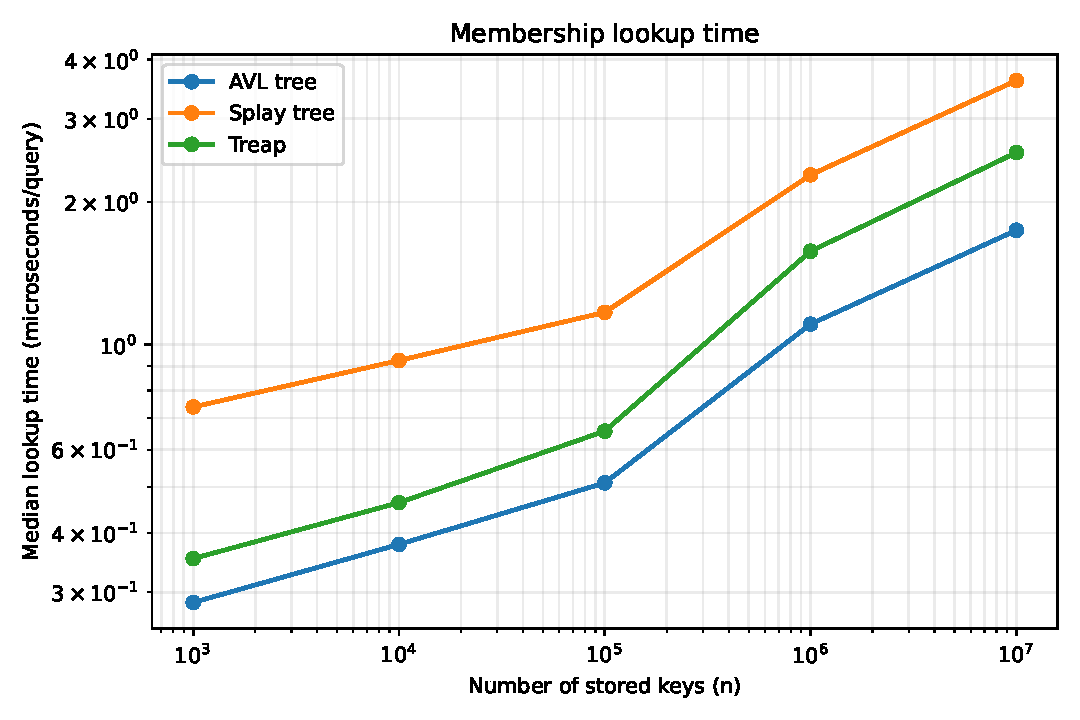
\includegraphics[width=.85\linewidth]{final_lookup_log.pdf}
\Description{Logarithmic plot of median membership lookup time for AVL, splay, and treap trees from one thousand to ten million stored keys.}
\caption{Median membership lookup time over 20,000 queries per fresh trial. Both axes are logarithmic.}
\label{fig:lookup}
\end{figure}

\begin{figure}[t]
\centering
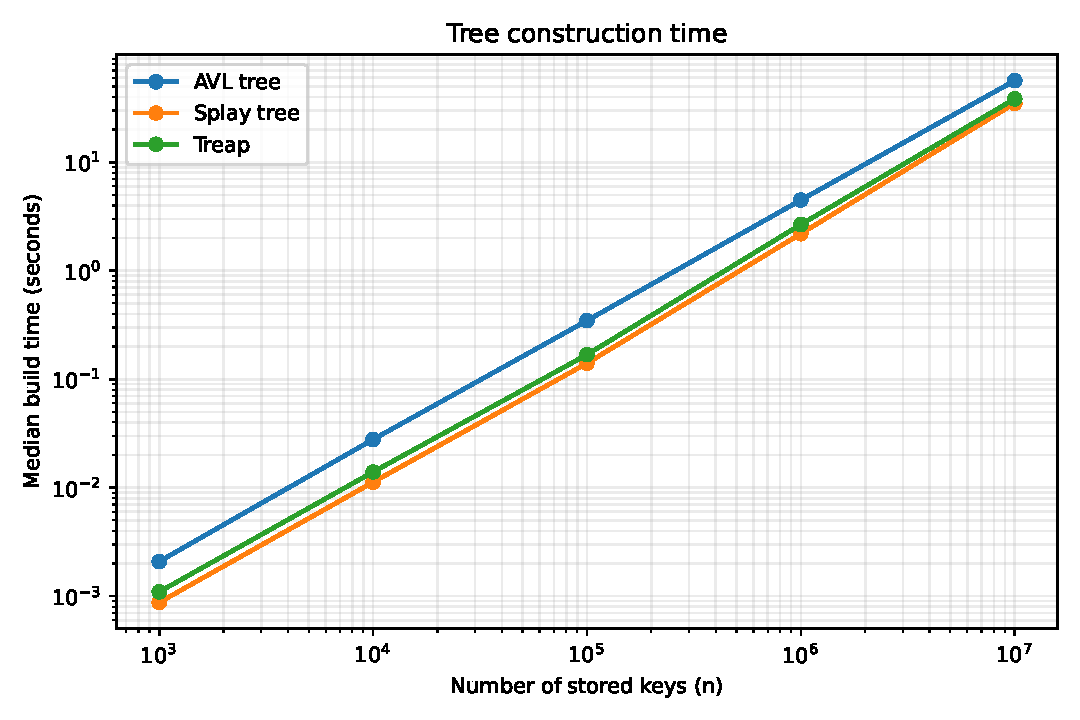
\includegraphics[width=.85\linewidth]{final_build.pdf}
\Description{Logarithmic plot of median construction time for AVL, splay, and treap trees from one thousand to ten million stored keys.}
\caption{Median time to insert all $n$ keys into an initially empty tree. Dataset generation is excluded.}
\label{fig:build}
\end{figure}

AVL has the fastest lookup at every measured size, followed by treap and then splay. At $n=10^7$, the median times are 1.744, 2.545, and 3.612 microseconds per query. Splay takes about 2.07 times as long as AVL on this workload, while treap takes about 1.46 times as long. These ratios describe the measured implementations, not their asymptotic bounds. AVL and treap lookups follow child pointers, while splay also rotates and reconnects nodes. For an absent query, splay moves a nearby stored key rather than the requested key.

Construction has a different ordering. At $n=10^7$, the median builds take 56.575 seconds for AVL, 34.937 seconds for splay, and 38.388 seconds for treap. AVL pays to maintain subtree heights and rebalance each insertion; its faster later lookup comes with higher build cost here. Splay's insertion restructures the tree too, but in this implementation it avoids stored height metadata and recursive insertion. Treap uses a priority per node and recursive rotations, yielding build time between the other two. A single run is influenced by allocation and cache behavior, so the three medians support a comparison on this machine rather than a universal ranking.

Increasing $n$ from one to ten million multiplies median build time by approximately 12.6 for AVL, 15.9 for splay, and 14.4 for treap. These values are reasonably compatible with $n\log n$-type growth plus changing memory costs. In the same step, median lookup time rises by only about 1.58, 1.58, and 1.62 times. The larger lookup jump between $10^5$ and $10^6$ for all three methods is plausible when the working set exceeds faster CPU caches; the experiment does not measure cache misses directly, so this remains an interpretation rather than a measured cause. No result contradicts the stated worst-case, amortized, or expected bounds: those bounds do not promise a specific constant or smooth finite-size curve.

\section{Discussion and Limitations}
The asymptotic bounds describe growth, not the ordering of measured constant factors. In particular, splaying performs rotations and pointer assignments even on membership queries, while AVL and treap lookups only descend. Conversely, splay can exploit repeated hot keys in a workload designed to have that locality; this experiment uses a mostly uniform mixed workload and does not establish its performance on a hot-key distribution. Treap's expected bound assumes random priorities, and its fixed seed gives one reproducible realization rather than averaging over independent priority seeds. AVL's worst-case bound follows from its height invariant regardless of the shuffled insertion order.

The build times include node allocation, comparisons, rotations, and Python overhead. Lookup times also include method-call and loop overhead. The plots do not prove an asymptotic bound. Peak memory was not measured: each tree stores $O(n)$ nodes, but Python's actual memory use depends on object layout and allocation. The 40 MB input array is extra benchmark storage, not part of a tree. The treap's theoretical expected bound assumes independent random priorities; this experiment uses one reproducible order from a seeded 64-bit generator. All three methods return exact membership answers, so there is no false-positive rate to report.

\section{Conclusion}
The comparison holds the keys, insertion order, and membership queries fixed while changing the tree's balancing policy. The three methods offer different kinds of logarithmic guarantees: AVL worst-case, splay amortized, and treap expected. The recorded measurements illustrate their practical costs on this workload, including the work done by splay queries to restructure the tree. The repository contains executable source, tests, the dataset manifest, raw CSVs, and plots so the experiment can be checked and rerun.

\section*{Repository and Dataset}
Source code: \url{https://github.com/rubenispiryan/cosc520-a2}.\par
Dataset: \url{https://github.com/rubenispiryan/cosc520-a2/blob/main/data/keys_n10000000_seed520.txt.gz}. The accompanying manifest records its seed and checksum.\par

\section*{Use of Generative AI}
% Final-state attribution: valid after the author rewrites all three tree implementations.
\begin{itemize}
\item \textbf{OpenAI Codex} assisted with dataset generation, benchmark and plotting scripts, unit tests, documentation, README, and report drafting.
\item \textbf{The author} selected the trees, wrote the final AVL, splay, and treap implementations, directed and reviewed the work, and takes responsibility for the personal selection reasons in Section 1.
\end{itemize}

\begin{thebibliography}{4}
\bibitem{nistavl} P. E. Black. AVL tree. \emph{Dictionary of Algorithms and Data Structures}, National Institute of Standards and Technology. \url{https://xlinux.nist.gov/dads/HTML/avltree.html}.
\bibitem{mitavl} MIT OpenCourseWare. 2011. Lecture 6: AVL Trees, AVL Sort. \url{https://courses.csail.mit.edu/6.006/fall11/lectures/lecture6.pdf}.
\bibitem{sleator1985} D. D. Sleator and R. E. Tarjan. 1985. Self-Adjusting Binary Search Trees. \emph{Journal of the ACM} 32, 3, 652--686. \url{https://www.cs.cmu.edu/~sleator/papers/Self-Adjusting.htm}.
\bibitem{seidel1996} R. Seidel and C. R. Aragon. 1996. Randomized Search Trees. \emph{Algorithmica} 16, 464--497. \url{https://faculty.washington.edu/aragon/pubs/rst96.pdf}.
\end{thebibliography}
\end{document}
